\chapter{Sets and Maps}
During the first term we have seen how important \blue{sets} and \blue{functional relations} are.  In the
following, functional relations will be called \blue{maps}.  In computer science, maps are also
known as \href{https://en.wikipedia.org/wiki/Associative_array}{\blue{associative arrays}}, 
\blue{dictionaries}, or \blue{symbol tables}.
In this chapter we show how sets and
maps can be implemented efficiently.  We confine our attention to the implementation of maps.  The
reason is that a set $M$ can always be represented by its \blue{characteristic function}:  If $M$ is
a set, then the characteristic function $\chi_M$ is defined such that
\\[0.2cm]
\hspace*{1.3cm}
$x \in M \Leftrightarrow \chi_M(x) = \mathtt{true}$
\\[0.2cm]
holds true.  In order to implement a set $M$ we can therefore implement its characteristic function
as a map.  The rest of this chapter is organized as follows:
\begin{enumerate}
\item We begin with the definition of the abstract data type of a \blue{map}.
    
      Following this definition we present several different implementations of maps. 
\item We start our discussion with \blue{ordered binary trees}.  These trees can be used to implement maps,
      provided the keys are ordered.        The average complexity of inserting
      an element into an ordered binary tree is \blue{logarithmic}.  Unfortunately, the worst case complexity
      is \blue{linear} in the number of the entries.
\item Next, we discuss \blue{balanced ordered trees}.  In the case of balanced ordered trees the
      complexity of insertion is g\underline{uaranteed} to be \blue{logarithmic}.
\item After that, we discuss so called \blue{tries}.  These can be used as maps if the keys to be
      stored in the map are \blue{strings}.
\item Finally, we discuss \blue{hash tables}.  Hash tables provide another way to implement a map.
      Although I personally think that hash tables are a bit overrated, they are in wide spread use
      and therefore every computer scientist should have a good understanding of their inner workings.
\end{enumerate}

\section{The Abstract Data Type \blue{Map}} 
Many applications require the efficient maintenance of some mapping of \blue{keys} to
\blue{values}.  For example, in order to implement a software analogue of a telephone book we have to
be able to associate the telephone numbers with the names.  In this case, the name of a person is regarded as a
\blue{key} and the telephone number is the \blue{value} that gets associated with the key.
The most important functions provided by a telephone directory are the following:
\begin{enumerate}
\item \blue{Lookup}: We have to be able to look up a given name and return the telephone number
      associated with this name.
\item \blue{Insertion}: We need to be able to insert a new name and the corresponding telephone
      number into our directory.
\item \blue{Deletion}: The final requirement is that it has to be possible to delete names from
      the directory.
\end{enumerate}


\begin{Definition}[Map] \hspace*{\fill} \\
{\em
  The abstract data type of a \blue{Map} is defined as follows:
  \begin{enumerate}
  \item The name is \textsl{Map}.
  \item The set of type parameters is $\{ \textsl{Key}, \textsl{Value} \}$.
  \item The set of function symbols is \\[0.1cm]
       \hspace*{1.3cm} 
       $\{ \textsl{map}, \textsl{find}, \textsl{insert}, \textsl{delete} \}$.
  \item The signatures of these function symbols are as follows:
        \begin{enumerate}
        \item $\textsl{map}: \textsl{Map}$

              Calling $\textsl{map}()$ generates a new empty map.  Here, an empty map is a map that
              does not store any keys.
        \item $\textsl{find}: \textsl{Map} \times \textsl{Key} \rightarrow \textsl{Value} \cup \{\Omega\}$

              The function call
              \\[0.2cm]
              \hspace*{1.3cm}
              $m.\textsl{find}(k)$ 
              \\[0.2cm]
              checks whether the key $k$ is stored in the map $m$.  If this is the case, the
              value associated with this key is returned, otherwise the function call returns
              the undefined value $\Omega$.
        \item $\textsl{insert}: \textsl{Map} \times \textsl{Key} \times \textsl{Value} \rightarrow \textsl{Map}$

              The function call
              \\[0.2cm]
              \hspace*{1.3cm}
              $m.\textsl{insert}(k,v)$ 
              \\[0.2cm]
              takes a key $k$ and an associated value $v$ and stores this information into the map
              $m$.  If the map $m$ already stores a value associated with the key $k$, this value
              is overwritten.  

              The function call returns the resulting map.
        \item $\textsl{delete}: \textsl{Map} \times \textsl{Key} \rightarrow \textsl{Map}$

              The function call
              \\[0.2cm]
              \hspace*{1.3cm}
              $m.\textsl{delete}(k)$ 
              \\[0.2cm]
              removes the key $k$ and any value associated with $k$ from the map $m$.  If the map $m$ does not contain a value for the
              key $k$, then the map is returned unchanged.

              The function call returns the new map. 
        \end{enumerate}
  \item The behaviour of a map is specified via the following axioms.
        \begin{enumerate}
        \item $\textsl{map}().\textsl{find}(k) = \Omega$.

              Calling $\textsl{map}()$ generates an empty map which does not have any keys stored.
              Hence, looking up any key in the empty map will just return the undefined value.
        \item $m.\textsl{insert}(k, v).\textsl{find}(k) = v$.

              If a value $v$ is inserted for a key $k$, then when we look up this key $k$ the corresponding value
              $v$ will be returned.
        \item $k_1 \not= k_2 \rightarrow m.\textsl{insert}(k_1, v).\textsl{find}(k_2) = m.\textsl{find}(k_2)$.

              If a value is inserted for a key $k_1$, then this does not change the value that is stored
              for any key $k_2$  different from $k_1$.
        \item $m.\textsl{delete}(k).\textsl{find}(k\bigr) = \Omega$.

              If the key $k$ is deleted, then afterwards we won't find this key anymore.
        \item $k_1 \not= k_2 \rightarrow 
               m.\textsl{delete}(k_1).\textsl{find}(k_2) = m.\textsl{find}(k_2)$,

              If  we delete a key $k_1$ and then try to look up the information stored under a key
              $k_2$ that is different from $k_1$, we will get the same result that we would have gotten
              if we had searched for $k_2$ before deleting $k_1$.
              \eox
        \end{enumerate}
  \end{enumerate}
}
\end{Definition}

In \textsl{Python} it is very easy to implement the abstract data type  \textsl{map}.  We just have
to realize that a map is essentially the same thing as a dictionary.
Now if $d$ is a dictionary storing the value $v$ for a key $k$, then the expression
\\[0.2cm]
\hspace*{1.3cm} $d[k]$
\\[0.2cm]
returns the value $v$.  On the other hand we can insert a value $v$ for a key $k$ by
writing
\\[0.2cm]
\hspace*{1.3cm}
$d[k] = v$ 
\\[0.2cm]
and in order to delete the value stored for a key  $k$ we can use the \texttt{del} statement
as follows: \\[0.2cm]
\hspace*{1.3cm} $\texttt{del}\ d[k]$. \\[0.2cm]
Figure  \ref{fig:Map-Trivial.ipynb} presents an implementation of the class \texttt{Map} that proceeds along
these lines.


\begin{figure}[!ht]
  \centering
\begin{minted}[ frame         = lines, 
                framesep      = 0.3cm,
                bgcolor       = sepia,
                numbers       = left,
                numbersep     = -0.2cm,
                xleftmargin   = 0.8cm,
                xrightmargin  = 0.8cm
              ]{python3}
    class Map:
        def __init__(self):
            self.mDictionary = {}
        
        def find(self, k):
            return self.mDictionary[k]
        
        def insert(self, k, v):
            self.mDictionary[k] = v
            
        def delete(self, k):
            del self.mDictionary[k]
            
        def __str__(self):
            return str(self.mDictionary)
\end{minted}
\vspace*{-0.3cm}
  \caption{A trivial implementation of the abstract data type \textsl{Map} in \textsl{Python}.}
  \label{fig:Map-Trivial.ipynb}
\end{figure} 
Note that the methods \texttt{insert} and \texttt{delete} do not return a object of type \texttt{Map}.  Rather, for
efficiency reasons, the existing \texttt{Map} is updated.


\section{Ordered Binary Trees}
If the set \textsl{Key} is linearly ordered, i.e.~if there exists a binary relation
$\leq \,\subseteq\,\textsl{Key}\times\textsl{Key}$ such that the pair $\langle \textsl{Key}, \leq \rangle$ is a linear
order, then the abstract data type \textsl{Map} can be implemented via  
\href{https://en.wikipedia.org/wiki/Binary_search_tree}{\blue{ordered binary trees}} also known as
\blue{binary search trees}. 
The implementation of the ADT map that is based on ordered binary trees has the following performance
characteristics: 
\begin{enumerate}
\item The average case complexity of the lookup operation is \blue{logarithmic}.
\item The worst case complexity of the lookup operation is \blue{linear}.  
\end{enumerate}
In order to define \blue{ordered binary trees} we introduce
\blue{binary trees} first.

\begin{Definition}[Binary Trees] \hspace*{\fill} \\
  Assume a set $\textsl{Key}$ and a set $\textsl{Value}$ are given.
  The set $\Bin$ of binary trees is defined inductively as the set of terms that is build using the
  function symbols \textsl{Nil} and \textsl{Node}, where the signature of these function symbols is
  given as follows: \\[0.2cm]
  \hspace*{1.3cm} 
  $\textsl{Nil}: \Bin$ \qquad and \qquad  $\textsl{Node}: \textsl{Key} \times \textsl{Value} \times \Bin \times \Bin \rightarrow \Bin$.
  \begin{enumerate}
  \item $\textsl{Nil}$ is a binary tree.

        This tree is called the \blue{empty tree} since it does not store any information.
  \item $\textsl{Node}(k, v, l, r)$ is a binary tree if the following holds true: 
        \begin{enumerate}
        \item $k$ is a key from the set $\textsl{Key}$.
        \item $v$ is a value from the set $\textsl{Value}$.
        \item $l$ is a binary tree.

              $l$ is the  \blue{left subtree} of the tree $\textsl{Node}(k, v, l, r)$.
        \item $r$ is a binary tree.

              $r$ is the \blue{right subtree} of the tree $\textsl{Node}(k, v, l, r)$.
              \eox
        \end{enumerate}
  \end{enumerate}
\end{Definition}

\noindent
Next, we define the notion of an  \blue{ordered binary tree}.
\begin{Definition}[Ordered Binary Tree] \hspace*{\fill} \\
  The set $\Bin_<$ of all \blue{ordered binary trees} is defined inductively.
  \begin{enumerate}
  \item $\textsl{Nil} \in \Bin_<$
  \item $\textsl{Node}(k, v, l, r) \in \Bin_<$ \quad iff the following conditions hold:
        \begin{enumerate}
        \item $k$ is a key from the set $\textsl{Key}$.
        \item $v$ is a value from the set $\textsl{Value}$.
        \item $l$ and $r$ are ordered binary trees.
        \item All keys that occur in the left subtree $l$ are smaller than $k$.
        \item All keys that occur in the right subtree $r$ are bigger than $k$.
        \end{enumerate}
        The last two conditions are known as the \blue{ordering conditions}.
        \eox
  \end{enumerate}
\end{Definition}
Graphically, ordered binary trees are depicted as follows:
\begin{enumerate}
\item The empty tree \textsl{Nil} is shown as a black circle.
\item A binary tree of the form $\textsl{Node}(k,v,l,r)$ is represented by an oval.  Inside of this
      oval, both the key $k$ and the value $v$ are printed.  The key is printed above the value and
      both are separated by a horizontal line.  This oval is then called a
      \blue{node} of the binary tree. 
      The left subtree $l$ of the node is depicted both to the left and  below the node,
      while the right subtree $r$ is depicted both to the right and below the node.  Both the left
      and the right subtree are connected to the node with an arrow that points from the node to the
      subtree.
\end{enumerate}
Figure \ref{fig:graph1} shows an example of an ordered binary tree.  The topmost node, that is the
node that has the key $8$ and the value $22$ is called the \blue{root} of the binary tree.
A \blue{path of length} $k$ in the tree is  list $[n_0,n_1, \cdots, n_k]$ of
$k+1$ nodes that are connected via arrows.  If we identify nodes with their labels, we have that
\\[0.2cm]
\hspace*{1.3cm} $\bigl[ \pair(8,22), \pair(12,18), \pair(10,16), \pair(9,39) \bigr]$ \\[0.2cm]
is a path of length 3.


\begin{figure}[!ht]
  \centering
  \framebox{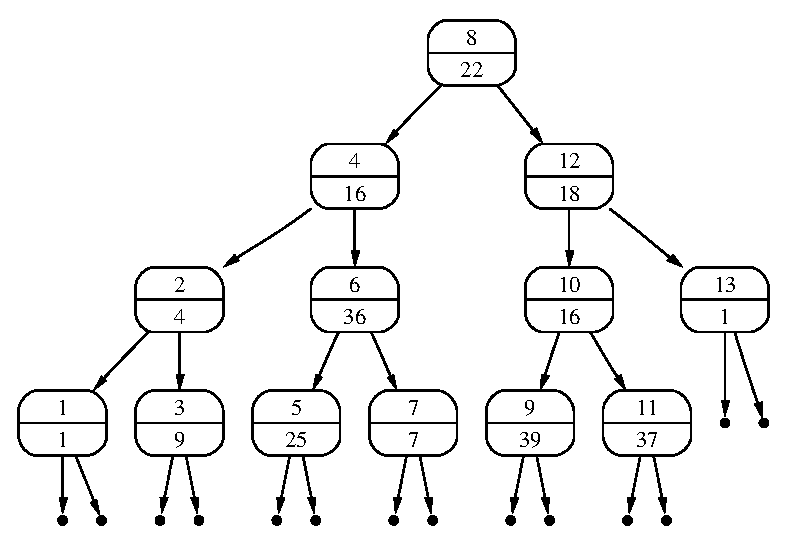
\epsfig{file=Abbildungen/graph1.eps}} 
  \caption{An ordered binary tree.}
  \label{fig:graph1}
\end{figure}


Next, we show how ordered binary trees can be used to implement the ADT  \textsl{Map}.  We specify
the different methods of this ADT via conditional equations.  The constructor $\textsl{map}()$
returns the empty tree:
\\[0.2cm]
\hspace*{1.3cm}
$\textsl{map}() = \textsl{Nil}$. 
\\[0.2cm]
The  method $\textsl{find}()$ is specified as follows:
\begin{enumerate}
\item $\textsl{Nil}.\textsl{find}(k) = \Omega$,

      because the empty tree is interpreted as the empty map.
\item $\textsl{Node}(k, v, l, r).\textsl{find}(k) = v$,

      because the node $\textsl{Node}(k,v,l,r)$ stores the assignment $k \mapsto v$.
\item $k_1 < k_2 \rightarrow \textsl{Node}(k_2, v, l, r).\textsl{find}(k_1) = l.\textsl{find}(k_1)$,

      because if $k_1$ is less than $k_2$, then any mapping for $k_1$ has to be stored in the left
      subtree  $l$.
\item $k_1 > k_2 \rightarrow \textsl{Node}(k_2, v, l, r).\textsl{find}(k_1) = r.\textsl{find}(k_1)$,

      because if $k_1$ is greater than $k_2$, then any mapping for $k_1$ has to be stored in the right
      subtree  $r$.
\end{enumerate}
Next, we specify the method  \textsl{insert}.  The definition of \textsl{insert} is similar to the
definition of the method  \textsl{find}.
\begin{enumerate}
\item $\textsl{Nil}.\textsl{insert}(k,v) = \textsl{Node}(k,v, \textsl{Nil}, \textsl{Nil})$,
  
      If the tree is empty, the information to be stored can be stored at the root.
\item $\textsl{Node}(k,v_2,l,r).\textsl{insert}(k,v_1) = \textsl{Node}(k, v_1, l, r)$,

      If the key $k$ is located at the root, we can just overwrite the old information. 
\item $k_1 < k_2 \rightarrow 
         \textsl{Node}(k_2, v_2, l, r).\textsl{insert}(k_1, v_1) = \textsl{Node}(k_2, v_2, l.\textsl{insert}(k_1, v_1), r)$,

      If the key $k_1$, which is the key for which we want to store a value, is less than the key
      $k_2$ at the root, then we have to insert the information in the left subtree.
\item $k_1 > k_2 \rightarrow 
         \textsl{Node}(k_2, v_2, l, r).\textsl{insert}(k_1, v_1) = 
         \textsl{Node}(k_2, v_2, l, r.\textsl{insert}(k_1, v_1))$,

      If the key $k_1$, which is the key for which we want to store a value, is bigger than the key
      $k_2$ at the root, then we have to insert the information in the right subtree.
\end{enumerate}
Finally we specify the method  \textsl{delete}.  The specification of \textsl{delete} is more
difficult than the specification of \textsl{find} and \textsl{insert}.
If there is a tree of the form $t =\textsl{Node}(k,v,l,r)$ and we want to delete the key $k$, then
we have to check first whether either of the subtrees  $l$ or $r$ is empty.  If $l$ is empty,
$t.\textsl{delete}(k)$ can return the right subtree  $r$ while if $r$ is empty,
$t.\textsl{delete}(k)$ can return the left subtree $l$.
Things get more difficult when both $l$ and $r$ are non-empty.  In this case,
our solution is that we look for the smallest key in the right subtree $r$.
This key and its corresponding value are removed from $r$.  The resulting tree is called $r'$.
Next, we take the node $t =\textsl{Node}(k,v,l,r)$ and transform it into the node
$t'=\textsl{Node}(k_{min},v_{min},l,r')$.  Here $k_{min}$ denotes the smallest key found in $r$ while
$v_{min}$ denotes the corresponding value.  Note that $t'$ is again ordered:
\begin{enumerate}
\item The key $k_{min}$ is bigger than the key $k$ and hence it is bigger than all keys in the left
      subtree $l$.
\item The key $k_{min}$ is smaller than all keys in the subtree  $r'$, because $k_{min}$ is the
      smallest key from the subtree $r$.
\end{enumerate}
In order to illustrate the idea, let us consider the following example: 
If we want to delete the node with the label  $\pair(4,16)$ from the tree shown in Figure
\ref{fig:graph1}, we first have to look for the smallest key in the subtree whose root is labelled
$\pair(6,36)$.  We find the node marked with the label $\pair(5,25)$.  We remove this node and
relabel the node that had the label $\pair(4,16)$ with the new label $\pair(5,25)$.  The result is
shown in Figure \ref{fig:graph2} on page \pageref{fig:graph2}.

\begin{figure}[!th]
  \centering
  \framebox{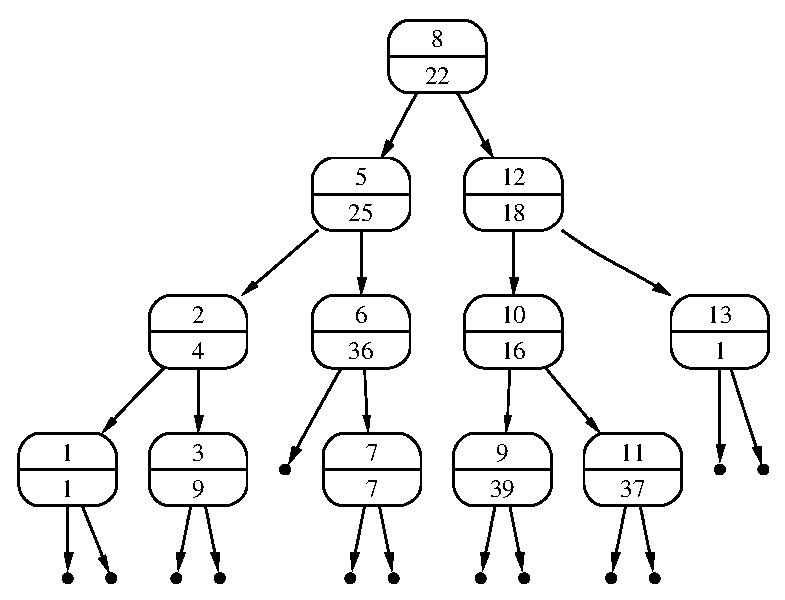
\epsfig{file=Abbildungen/graph2.eps}} 
  \caption{The ordered binary tree from Figure  
          \ref{fig:graph1} after deleting the node with label $\pair(4,16)$.}
  \label{fig:graph2}
\end{figure}

Next, we specify the  method \textsl{delMin}.  The call $t.\textsl{delMin}()$ returns a triple.
If 
\\[0.2cm]
\hspace*{1.3cm}
$t.\textsl{delMin}() = [r,k,v]$,
\\[0.2cm]
then $r$ is the tree that  results from
removing the smallest key in $t$, $k$ is the key that is removed and $v$ is the associated value.
\begin{enumerate}
\item $\textsl{Node}(k, v, \textsl{Nil}, r).\textsl{delMin}() = [r, k, v]$

      If the left subtree is empty, $k$ has to be the smallest key in the tree 
      $\textsl{Node}(k, v, \textsl{Nil}, r)$.  If $k$ is removed, we are left with the subtree $r$.
\item $l\not= \textsl{Nil} \wedge l.\textsl{delMin}() = [l',k_{min}, v_{min}] \;\rightarrow$ \\[0.2cm]
       \hspace*{1.3cm} 
       $\textsl{Node}(k, v, l, r).\textsl{delMin}() = [\textsl{Node}(k, v, l', r), k_{min}, v_{min}]$.

      If the left subtree $l$ in the binary tree $t = \textsl{Node}(k, v, l, r)$
      is not empty, then the smallest key of  $t$ is located inside the left subtree $l$.
      This smallest key is recursively removed from  $l$. This yields the tree 
      $l'$.  Next,  $l$ is replaced by $l'$ in $t$.  The resulting tree is
      $t' = \textsl{Node}(k, v, l', r)$.
\end{enumerate}
Next, we specify the method $\mathtt{delete}()$.
\begin{enumerate}
\item $\textsl{Nil}.\textsl{delete}(k) = \textsl{Nil}$.
\item $\textsl{Node}(k,v,\textsl{Nil},r).\textsl{delete}\bigl(k\bigr) = r$.
\item $\textsl{Node}(k,v,l,\textsl{Nil}).\textsl{delete}(k) = l$.
\item $l \not= \textsl{Nil} \,\wedge\, r \not= \textsl{Nil} \,\wedge\, r.\textsl{delMin}() = [r',k_{min}, v_{min}]  \;\rightarrow$ \\[0.2cm]
      \hspace*{1.3cm}
      $\textsl{Node}(k,v,l,r).\textsl{delete}(k) = \textsl{Node}(k_{min},v_{min},l,r')$.
      
      If the key to be removed is found at the root of the tree and neither of its subtrees is
      empty, the call  $r\mathtt{.}\textsl{delMin}()$ removes the smallest key together with its
      associated value from the subtree $r$ yielding the subtree $r'$.
      The smallest key from $r$ is then stored at the root of the new tree.

\item $k_1 < k_2 \rightarrow \textsl{Node}(k_2,v_2,l,r).\textsl{delete}\bigl(k_1) = 
       \textsl{Node}(k_2,v_2,l.\textsl{delete}(k_1),r)$.

       If the key that is to be removed is less than the key stored at the root, the key $k$ can only be
       located in the left subtree $l$.  Hence, $k$ is removed from the left subtree $l$ recursively.
\item $k_1 > k_2 \rightarrow \textsl{Node}(k_2,v_2,l,r).\textsl{delete}(k_1) = 
       \textsl{Node}(k_2,v_2,l,r.\textsl{delete}(k_1))$.

       If the key that is to be removed is greater than the key stored at the root, the key $k$ can only be
       located in the right subtree $r$.  Hence, $k$ is removed from the right subtree $r$ recursively.
\end{enumerate}

\subsection{Implementing Ordered Binary Trees in \textsl{Python}}
Figure \ref{fig:binary-tree.stlx-1} and Figure \ref{fig:binary-tree.stlx-2} show how ordered binary
trees can be implemented in \textsl{Python}.  Objects of class \texttt{map} encapsulate ordered
binary trees.  We discuss the implementation of this class next.
\begin{enumerate}
\item The constructor map is called with one argument.  This argument, called \texttt{cmp}
      in line 1, is a function representing a total order ''$<$''.  The idea is that the function
      \texttt{cmp} is called with two arguments and we have
      \\[0.2cm]
      \hspace*{1.3cm}
      $\mathtt{cmp}(x,y)$ \quad if and only if \quad $x < y$.
      \\[0.2cm]
      The function \texttt{cmp} is later stored in the member variable \texttt{mCmpFct} in line 6.
\item The class \texttt{map} represents a node in an ordered binary tree.  In order to do so, it
      maintains four additional member variables.
      \begin{enumerate}
      \item \texttt{mKey} is the key stored at this node.  For an empty node, \texttt{mKey}
            has the value \texttt{om}, which represents $\Omega$.
      \item \texttt{mValue} stores the value that is associated with \texttt{mKey}.  For an empty node,
            \texttt{mValue} is \texttt{om}.
      \item \texttt{mLeft} is the left subtree.  An empty subtree is represented as \texttt{om}.
      \item \texttt{mRight} is the right subtree.  
      \end{enumerate}
\item The function \texttt{isEmpty} checks whether \texttt{this} represents an empty tree.
      The assumption is that if \texttt{mKey} is \texttt{om}, then the member variables
      \texttt{mValue}, \texttt{mLeft}, and \texttt{mRight} will also be \texttt{om}.
\item The implementation of \texttt{find} works as follows:
      \begin{enumerate}
      \item If the node is empty, there is no value to find and the function returns \texttt{om}.
            Note that in \textsl{Python} a \texttt{return} statement which does not return a value 
            automatically returns \texttt{om}.
      \item If the key we are looking for is stored at the root of this tree, the value stored for
            this key is \texttt{mValue}.
      \item Otherwise, we have to compare the key \texttt{k}, which is the key we are looking for,
            with the key \texttt{mKey}, which is the key stored in this node.  If \texttt{k}
            is less than \texttt{mKey}, \texttt{k} can only be stored in the left subtree
            \texttt{mLeft}, while if $k$ is greater than \texttt{mKey}, \texttt{k} can only be
            stored in the right subtree.
      \end{enumerate}


\begin{figure}[!ht]
  \centering
\begin{Verbatim}[ frame         = lines, 
                  framesep      = 0.3cm, 
                  labelposition = bottomline,
                  numbers       = left,
                  numbersep     = -0.2cm,
                  xleftmargin   = 0.0cm,
                  xrightmargin  = 0.0cm
                ]
    class map(cmp) {
        mKey    := om;
        mValue  := om; 
        mLeft   := om;
        mRight  := om;
        mCmpFct := cmp;  // function to compare keys
      static {
        isEmpty := [] |-> mKey == om;
        find := procedure(k) {
            if      (isEmpty())        { return;                }
            else if (mKey == k)        { return mValue;         }
            else if (mCmpFct(k, mKey)) { return mLeft .find(k); }
            else                       { return mRight.find(k); }
        };
        insert := procedure(k, v) {
              if (isEmpty()) { 
                this.mKey   := k;
                this.mValue := v; 
                this.mLeft  := map(mCmpFct);
                this.mRight := map(mCmpFct);
            } else if (mKey == k) { 
                mValue := v; 
            } else if (mCmpFct(k, mKey)) { 
                mLeft .insert(k, v); 
            } else { 
                mRight.insert(k, v); 
            }
        };
\end{Verbatim}
\vspace*{-0.3cm}
  \caption{Implementation of ordered binary trees \textsl{Python}, part (I).}
  \label{fig:binary-tree.stlx-1}
\end{figure}
\item The implementation of \texttt{insert} is similar to the implementation of \texttt{find}.
      \begin{enumerate}
      \item If the binary tree is empty, we set the member variables \texttt{mKey} and
            \texttt{mValue} to the appropriate values.  The member variables \texttt{mLeft} and 
            \texttt{mRight} are initialized as empty trees.
      \item If the key \texttt{k} under which the value \texttt{v} is to be inserted is identical
            to the key \texttt{mKey} stored at this node, then we have found the node where we need
            to insert \texttt{v}.  In this case, \texttt{mValue} is overwritten with \texttt{v}.
      \item Otherwise, \texttt{k} is compared with \texttt{mKey} and the search is continued in the
            appropriate subtree.
      \end{enumerate}      


\begin{figure}[!ht]
  \centering
\begin{Verbatim}[ frame         = lines, 
                  framesep      = 0.3cm, 
                  firstnumber   = last,
                  labelposition = bottomline,
                  numbers       = left,
                  numbersep     = -0.2cm,
                  xleftmargin   = 0.8cm,
                  xrightmargin  = 0.8cm
                ]
        delMin := procedure() {
            if (mLeft.isEmpty()) { 
                return [ mRight, mKey, mValue ]; 
            } else {
                 [ ls, km, vm ] := mLeft.delMin();
                 this.mLeft := ls;
                 return [ this, km, vm ];
            }
        };
        delete := procedure(k) {
            if      (isEmpty())  { return; } 
            else if (k == mKey)  {
                if      (mLeft .isEmpty()) { update(r); }  
                else if (mRight.isEmpty()) { update(l); } 
                else {
                    [ rs, km, vm ] := mRight.delMin();
                    this.mKey   := km;
                    this.mValue := vm; 
                    this.mRight := rs;
                }
            } else if (mCmpFct(k, mKey)) {
                if (!mLeft .isEmpty()) { mLeft .delete(k); }
            } else {
                if (!mRight.isEmpty()) { mRight.delete(k); }
            }
        };
        update := procedure(t) {
            this.mKey   := t.mKey;
            this.mValue := t.mValue;
            this.mLeft  := t.mLeft;
            this.mRight := t.mRight;
        };
      }
    }
\end{Verbatim}
\vspace*{-0.3cm}
  \caption{Implementation of ordered binary trees in \textsl{Python}, part (II).}
  \label{fig:binary-tree.stlx-2}
\end{figure}

\item The implementation of \texttt{delMin} and \texttt{delete} is done in a similar way as the
      implementation of \texttt{insert}.  It should be noted that the implementation follows directly from the
      equations derived  previously. 
      
      There is however one caveat that should be mentioned.  Line 55 show the implementation of the
      function \texttt{update}.  When we delete the key at the root of the tree and either of the
      subtrees is empty, we would ideally just overwrite the current tree with the non-empty
      subtree, i.e.~we would like to write something like
      \\[0.2cm]
      \hspace*{1.3cm}
      \texttt{this := mLeft;}
      \\[0.2cm]
      However, we cannot change the object \texttt{this}.  The only thing we can do is change the
      attributes of the object \texttt{this}.  This is done in the method \texttt{update}.
\end{enumerate}

\begin{figure}[!th]
  \centering 
  \framebox{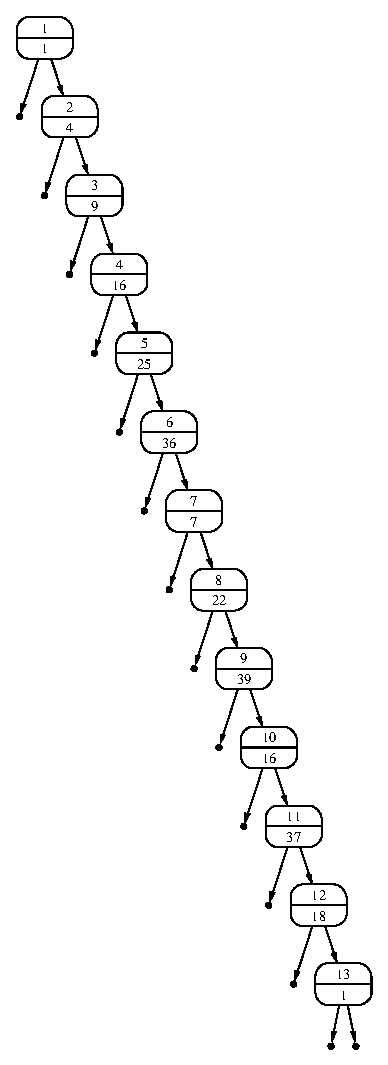
\epsfig{file=Abbildungen/degenerated-bin-tree}} 
  \caption{A degenerated binary tree.}
  \label{fig:degenerated}
\end{figure}


\subsection{Analysis of the Complexity}
In this section we will first discuss the worst case complexity, which is quite bad.  In fact, in
the worst case, the call $b.\mathtt{find}(k)$ will perform $\Oh(n)$ key comparisons if $b$ is an ordered
binary search tree of $n$ elements.  After that, we investigate the average case complexity.  We
will show that the average case complexity is $\Oh\bigr(\ln(n)\bigr)$.

\subsubsection{Worst Case Complexity}
We begin our investigation of the complexity with an analysis of the complexity of $b.\textsl{find}(k)$ 
in the worst case.  The worst case happens if the binary tree $b$ degenerates into a list.
Figure \ref{fig:degenerated} on page \pageref{fig:degenerated} shows the ordered binary tree that
is generated if the keys are inserted in increasing order.  If we then have to search for the
biggest key, we have to traverse the complete tree in order to find this key.  Therefore, if the
tree $b$ contains $n$ different keys, we have to compare the key $k$ that we are looking for to all
of these $n$ keys in the tree.  Hence, in this case the complexity of $b.\textsl{find}(k)$ is 
$\Oh(n)$ and this is the same complexity that we would have gotten if we had used a linked list.


\subsubsection{Average Case Complexity}
Fortunately, the worst case has a very small probability to occur. On average, a randomly generated
binary tree is quite well balanced.  We will show next that the number of comparisons necessary for
the function call $b.\textsl{find}(k)$ has the order $\Oh\bigl(\ln(n)\bigr)$.  


%Dazu definieren wir auf bin\"aren B\"aumen zun\"achst eine Funktion 
%\[ \textsl{height}: \Bin \rightarrow \N, \]
%die die H\"ohe eines bin\"aren Baums angibt.  Die Definition erfolgt induktiv.
%\begin{enumerate}
%\item $\textsl{Nil}.\textsl{height}() = 0$.

%      Der leere Baum hat die H\"ohe $0$.
%\item $\textsl{node}(k,v,l,r).\textsl{height}() = 
%       1 + \max\bigl(l.\textsl{height}(),\, r.\textsl{height}()\bigr)$.

%      Die H\"ohe des Baums $\textsl{node}(k,v,l,r)$ ist um eins gr\"o{\ss}er als die H\"ohe des
%      gr\"o{\ss}ten Teilbaums.
%\end{enumerate}
%Analog definieren wir f\"ur einen bin\"aren Baum $b$ die Anzahl $b.\textsl{count}()$ der Schl\"ussel, die
%der Baum enth\"alt.   Die Definition von $b.\textsl{count}()$ erfolgt durch Induktion nach $b$.
%\begin{enumerate}
%\item $\textsl{Nil}.\textsl{count}() = 0$.

%      Der leere Baum enth\"alt keine Schl\"ussel.
%\item $\textsl{node}(k,v,l,r).\textsl{count}() = 
%       1 + l.\textsl{count}() + r.\textsl{height}()\bigr)$.

%      Der Baum $\textsl{node}(k,v,l,r)$ enth\"alt zus\"atzlich zu dem Schl\"ussel $k$ die
%      Schl\"ussel aus den Teilb\"aumen $l$ und $r$.
%\end{enumerate}
%Der folgende Satz zeigt, wieviel Schl\"ussel ein Baum der H\"ohe $h$ h\"ochstens enthalten
%kann.

%\begin{Satz}
%  Ein bin\"arer Baum $b$ der H\"ohe $h$ enth\"alt h\"ochstens $2^h - 1$ Schl\"ussel.
%\end{Satz}
%\noindent
%\textbf{Beweis}:  Wir bezeichnen die maximale Anzahl Schl\"ussel eines Baums der H\"ohe $h$
%mit $c_h$.  Wir beweisen  durch Induktion nach $h$, dass gilt:
%\[ c_h = 2^h - 1. \]
%\begin{enumerate}
%\item[I.A.] $h = 0$: Der einzige Baum der H\"ohe $0$ ist $\textsl{Nil}$.
%            Dieser enth\"alt $0$ Schl\"ussel.  Also gilt
%            \\[0.2cm]
%            \hspace*{1.3cm}
%            $c_0 = 0 = 2^0 - 1$.
%\item[I.S.] $h \mapsto h + 1$: Ein Baum der H\"ohe $h+1$, der die maximale Anzahl
%            Schl\"ussel enth\"alt, hat die Form $\textsl{node}(k,v,l,r)$, wobei dann $l$ und
%            $r$  B\"aume der H\"ohe $h$ sind, die die maximale Anzahl Schl\"ussel enthalten.
%            Folglich gilt:
%            \begin{eqnarray*}
%               c_{h+1} &               =  & 1 + c_h + c_h \\
%                       & \stackrel{IV}{=} & 1 + (2^h - 1) + (2^h - 1) \\
%                       &               =  & 2 \cdot 2^h - 1 \\
%                       &               =  & 2^{h+1} - 1. \hspace*{9cm} \Box
%            \end{eqnarray*}
%\end{enumerate}

%Die H\"ohe eines Baumes gibt ein Ma{\ss} f\"ur die Komplexit\"at der Methoden \textsl{find},
%\textsl{insert} und \textsl{delete}, denn bei einem Baum der H\"ohe $h$ sind f\"ur jede dieser
%Operationen h\"ochstens $h$ Vergleiche von Schl\"usseln erforderlich.

In order to prove this claim, we have to introduce some definitions.
We define the \underline{avera}g\underline{e} number of comparisons that are needed for the function
call $b.\textsl{find}(k)$ as  $d_n$, where $n$ is the number of keys stored in $b$.  We assume that
the key $k$ is indeed stored in $b$.  Our first goal is to derive a recurrence equation for 
$d_n$.  First, we note that  
\\[0.2cm]
\hspace*{1.3cm} $d_1 = 1$,
\\[0.2cm]
because if the tree $b$ contains only one key we will do exactly one key comparison.
Next, imagine a binary tree $b$ that contains $n+1$ keys.  Then $b$
can be written as 
\\[0.2cm]
\hspace*{1.3cm}
$b = \textsl{node}(k',v,l,r)$,
\\[0.2cm]
where $k'$ is the key at the root of $b$.  If the keys of $b$ are ordered as a list, then this
ordering looks something like the following:
\\[0.2cm]
\hspace*{1.3cm}
$k_0 < k_1 < \cdots < k_{i-1} < k_{i} < k_{i+1} < \cdots < k_{n-1} < k_n$.
\\[0.2cm]
Here, there are $n+1$ positions for the key $k'$.
If we have $k' = k_i$, then the left subtree of $b$ contains  $i$ keys while the right subtree
contains the remaining  $n-i$ keys:
\\[0.2cm]
\hspace*{1.3cm}
$\underbrace{k_0 < k_1 < \cdots < k_{i-1}}_{\mbox{keys in $l$}} < 
 \underbrace{k_{i}}_{\stackrel{\displaystyle \shortparallel}{\displaystyle k'}} < 
 \underbrace{k_{i+1} < \cdots < k_{n-1} < k_n}_{\mbox{keys in $r$}}$,
\\[0.2cm]
As  $b$ contains $n+1$ keys all together, there are  $n+1$ different possibilities for the position
of $k'$, as the number of keys in the left subtree $l$ is $i$ where
\\[0.2cm]
\hspace*{1.3cm}
 $i \in \{0,1, \cdots, n\}$.
\\[0.2cm]
Of course, if the left subtree has $i$ keys, the right subtree will have $n-i$ keys.
Let us denote the average number of comparisons that are done during the function call
$b.\textsl{find}(k)$ provided the left subtree of $b$ has $i$ keys while $b$ itself has $n+1$ keys
as
\\[0.2cm]
\hspace*{1.3cm}
$\textsl{numCmp}(i,\, n\!+\!1)$.
\\[0.2cm]
Then, since all values of $i$ have the same probability, we have
\\[0.2cm]
\hspace*{1.3cm}
$\ds d_{n+1} =  \frac{1}{n+1} \cdot \sum\limits_{i=0}^n \textsl{numCmp}(i,\, n\!+\!1)$.
\\[0.2cm]
We proceed to compute $\textsl{numCmp}(i,n\!+\!1)$:
If  $l$ contains $i$ keys while $r$ contains the remaining $n-i$ keys,
then there are three possibilities for the key $k$ that we want to find in $b$:
\begin{enumerate}
\item $k$ might be identical with the key $k'$ that is located at the root of $b$.
      In this case there is only one comparison.
      As there  are $n+1$ keys in $b$ and the key we are looking for will be at the root in only
      one of these cases, the probability of this case is
      \\[0.2cm]
      \hspace*{1.3cm} $\bruch{1}{\,n+1\,}$.

\item $k$ might be identical to one of the  $i$ keys of the left subtree $l$.
      The probability for this case is 
      \\[0.2cm]
      \hspace*{1.3cm} $\displaystyle\bruch{i}{n+1}$. \\[0.2cm]
      In this case we need 
      \\[0.2cm]
      \hspace*{1.3cm} $\displaystyle d_i + 1$ \\[0.2cm]
      comparisons because in addition to the  $d_i$ comparisons in the left subtree we have to
      compare the key $k$ we are looking for with the key $k'$ at the root of the tree.
\item $k$ might be a key in the right subtree $r$.  As there are  $n-i$ keys in the right subtree
      and the total of keys is $n+1$, the probability that the key  $k$ occurs in the right subtree $r$
      is \\[0.2cm]
      \hspace*{1.3cm} $\displaystyle \bruch{n-i}{n+1}$. \\[0.2cm]
      Hence, in this case there are  \\[0.2cm]
      \hspace*{1.3cm} $\displaystyle d_{n-i} + 1$ \\[0.2cm]
      comparisons. 
\end{enumerate}
In order to compute  $\textsl{numCmp}(i, n\!+\!1)$ we have to multiply the probabilities in every
case with the number of comparisons and these three numbers have to added.  This yields
\begin{eqnarray*}
  \textsl{numCmp}(i, n\!+\!1) 
& = & \bruch{1}{\,n+1\,} \cdot 1 + \bruch{i}{n+1} \cdot (d_i + 1) + \bruch{n-i}{n+1} \cdot (d_{n-i} + 1) 
      \\[0.2cm]
& = & \bruch{1}{\,n+1\,} \cdot \bigl(1 + i \cdot (d_i + 1) + (n-i) \cdot (d_{n-i} + 1)\bigr)      \\[0.2cm]
& = & \bruch{1}{\,n+1\,} \cdot \bigl(1 + i + (n-i) + i \cdot d_i + (n-i) \cdot d_{n-i} \bigr)    \\[0.2cm]
& = & \bruch{1}{\,n+1\,} \cdot \bigl(n + 1 + i \cdot d_i + (n-i) \cdot d_{n-i} \bigr)            \\[0.2cm]
& = & 1 + \bruch{1}{\,n+1\,} \cdot \bigl(i \cdot d_i + (n-i) \cdot d_{n-i} \bigr) 
\end{eqnarray*}


Therefore, the recurrence equation for $d_{n+1}$ is given as follows: 
\\[0.2cm]
\hspace*{1.3cm}
$
\begin{array}{lcl}
d_{n+1} 
& = &  
\ds\sum\limits_{i=0}^n \bruch{1}{\,n+1\,} \cdot \textsl{numCmp}(i,\,n\!+\!1)  \\[0.5cm]
& = &  
\ds\bruch{1}{n+1} \cdot \sum\limits_{i=0}^n  
           \left(1 + \bruch{1}{n+1} \cdot \bigl(i \cdot d_i + (n-i) \cdot d_{n-i} \bigr) \right)
\\[0.5cm]
& = &  
\bruch{1}{n+1} \cdot \Biggl(\underbrace{\sum\limits_{i=0}^n 1}_{\stackrel{\displaystyle \shortparallel}{n+1}} \;+\;
           \bruch{1}{n+1} \cdot \ds\sum\limits_{i=0}^n \bigl(i \cdot d_i + (n-i) \cdot d_{n-i} \bigr) \Biggr)
\\[1.3cm]
& = &  
1 + \bruch{1}{(n+1)^2} \cdot \left(\ds\sum\limits_{i=0}^n \left(i\cdot d_i + (n-i)\cdot d_{n-i}\right) \right) 
\\[0.5cm]
& = &  
1 + \bruch{2}{(n+1)^2} \cdot \ds\sum\limits_{i=0}^n i\cdot d_i 
\end{array}
$
\\[0.2cm]
Here we have used the equation  \\[0.2cm]
\hspace*{1.3cm}
$\ds\sum\limits_{i=0}^n f(n-i) = \sum\limits_{i=0}^n f(i)$. \\[0.2cm]
We had verified this equation already when discussing the complexity of Quick Sort in the average
case.  Next, we solve the recurrence equation 
\begin{equation}
  \label{eq:bin1}
d_{n+1} = \displaystyle 1 + \bruch{2}{(n+1)^2} \cdot \sum\limits_{i=0}^n i\cdot d_i  
\end{equation}
with the initial condition $d_1 = 1$.  
In order to solve the equation (\ref{eq:bin1}) we perform the substitution $n \mapsto n+1$.  This yields
\begin{equation}
  \label{eq:bin2}
d_{n+2} = \displaystyle 1 + \bruch{2}{(n+2)^2} \cdot \sum\limits_{i=0}^{n+1} i\cdot d_i  
\end{equation}
We multiply equation (\ref{eq:bin1}) with $(n+1)^2$ and equation (\ref{eq:bin2}) 
with $(n+2)^2$.  We get
\begin{eqnarray}
  \label{eq:bin3}
(n+1)^2 \cdot d_{n+1} & = & (n+1)^2 + 2 \cdot \sum\limits_{i=0}^n i\cdot d_i, \\
  \label{eq:bin4}
(n+2)^2 \cdot d_{n+2} & = & (n+2)^2 + 2 \cdot \sum\limits_{i=0}^{n+1} i\cdot d_i
\end{eqnarray}
We subtract equation  (\ref{eq:bin3}) from equation (\ref{eq:bin4})
and are left with \\[0.2cm]
\hspace*{1.3cm} 
$(n+2)^2 \cdot d_{n+2} - (n+1)^2 \cdot d_{n+1} = (n+2)^2 - (n+1)^2 + 2 \cdot (n+1) \cdot d_{n+1}$.
\\[0.2cm]
To simplify this equation we substitute  $n \mapsto n - 1$ and get \\[0.2cm]
\hspace*{1.3cm} 
$(n+1)^2 \cdot d_{n+1} - n^2 \cdot d_{n} = (n+1)^2 - n^2 + 2 \cdot n \cdot d_{n}$.
\\[0.2cm]
This can be simplified as \\[0.2cm]
\hspace*{1.3cm} $(n+1)^2 \cdot d_{n+1}  =  n \cdot (n + 2) \cdot d_{n} + 2 \cdot n + 1$. \\[0.2cm]
Let us divide both sides of this equation by $(n+2)\cdot (n+1)$.  We get \\[0.2cm]
\hspace*{1.3cm}  
$\displaystyle \bruch{n+1}{n+2} \cdot d_{n+1}  =  \bruch{n}{n + 1} \cdot d_{n} + \bruch{2 \cdot n + 1}{(n+2)\cdot (n+1)}$. \\[0.2cm]
We define \\[0.2cm]
\hspace*{1.3cm} $\displaystyle c_n = \bruch{n}{n+1} \cdot d_n$. \\[0.4cm]
Then $c_1 = \bruch{1}{2} \cdot d_1 = \bruch{1}{2}$ and hence we have found the recurrence equation \\[0.2cm]
\hspace*{1.3cm} 
$\displaystyle c_{n+1}  =  c_{n} + \frac{2 \cdot n + 1}{(n+2)\cdot (n+1)}$. \\[0.2cm]
A partial fraction decomposition shows \\[0.2cm]
\hspace*{1.3cm} 
$\displaystyle \frac{2 \cdot n + 1}{(n+2)\cdot (n+1)} = \frac{3}{n+2} - \frac{1}{n+1}$. \\[0.2cm]
Hence we have \\[0.2cm]
\hspace*{1.3cm} $\displaystyle c_{n+1} = c_n +  \frac{3}{n+2} - \frac{1}{n+1}$. \\[0.2cm]
Because of $c_1 = \bruch{1}{2}$ this equation is also valid for  $n=0$ if we define $c_0 = 0$, since
we have
\\[0.2cm]
\hspace*{1.3cm}
$\bruch{1}{2} = 0 + \bruch{3}{0+2} - \bruch{1}{0+1}$.
\\[0.2cm]
The recurrence equation for $c_n$ can be solved using  telescoping:
\begin{eqnarray*}  
  c_{n+1} & = & c_0 + \sum\limits_{i=0}^{n} \frac{3}{i+2} - \sum\limits_{i=0}^{n} \frac{1}{i+1} 
\\[0.2cm]
          & = & \sum\limits_{i=2}^{n+2} \frac{3}{i} - \sum\limits_{i=1}^{n+1} \frac{1}{i}.
\end{eqnarray*}
To simplify this equation we substitute $n \mapsto n-1$ and get
\\[0.2cm]
\hspace*{1.3cm}
$c_{n} =  \displaystyle\sum\limits_{i=2}^{n+1} \frac{3}{i} - \sum\limits_{i=1}^{n} \frac{1}{i}$
\\[0.2cm]
The harmonic number  $H_n$ is defined as 
$H_n = \ds\sum\limits_{i=1}^{n} \bruch{1}{i}$.   
Therefore,  $c_n$ can be reduced to $H_n$: 
\\[0.2cm]
\hspace*{1.3cm}
$c_n = \ds 3 \cdot H_n - \frac{3}{1} + \frac{3}{n+1} - H_n  =  \ds 2 \cdot H_n - 3 \cdot \frac{n}{n+1}$
\\[0.2cm] 
Because $H_n = \displaystyle\sum\limits_{i=1}^{n} \frac{1}{i} = \ln(n) + \Oh(1)$ and $\ds 3 \cdot\frac{n}{n+1} \in \Oh(1)$
we therefore have
  \\[0.3cm]
\hspace*{1.3cm} 
$\displaystyle c_n = 2 \cdot \ln(n) + \Oh(1)$.
\\[0.3cm]
Because of  $d_n = \bruch{n+1}{n}\cdot c_n$ we have \\[0.2cm]
\hspace*{1.3cm}
 $\displaystyle d_n = 2 \cdot \ln(n) + \Oh\bigl(1\bigr)$.
\\[0.2cm]
This is our main result:  On average, the operation $b.\textsl{find}(k)$ uses
\\[0.2cm]
\hspace*{1.3cm}
$2 \cdot \ln(n) = 2 \cdot \ln(2) \cdot \log_2(n) \approx 1.386 \cdot \log_2(n)$ 
\\[0.2cm]
comparisons.  Hence in the average case there are about  39 \% 
more comparisons than there would be if the tree was optimally balanced.
There are similar results for the operations \textsl{insert} and \textsl{delete}.


%%% Local Variables: 
%%% mode: latex
%%% TeX-master: "algorithms"
%%% End: 
